\section{Results}

\subsection{Open-loop prediction}

Table~\ref{tab:open-loop} summarizes the cell-balanced confirmatory results.
At 25 steps, CFR-WM obtains NRMSE $\CFRNRMSE$ versus $\PGNNNRMSE$ for the
preselected PGNN-style comparator. The paired seed-level relative improvement
is \PrimaryImprovement\% (95\% fixed-cell bootstrap interval
[\PrimaryRelativeCILow\%, \PrimaryRelativeCIHigh\%]); the exact one-sided
sign-flip test against the 5\% practical margin gives
$p=\PrimaryPValue$. The corresponding absolute difference is
\PrimaryDifference{} (95\% interval [\PrimaryCILow,
\PrimaryCIHigh]). These quantities satisfy the predeclared aggregate
criterion.

\begin{table*}[!t]
  \caption{Open-loop prediction over five systems, three regimes, and eight
  paired seeds. Entries are mean $\pm$ SD across seed-level cell-balanced
  aggregates.}
  \label{tab:open-loop}
  \centering
  \footnotesize
  \begin{tabular}{lrrrr}
\toprule
Method & Mean parameters & NRMSE-1 & NRMSE-10 & NRMSE-25 \\
\midrule
CFR-WM & 57694 & 0.039 $\pm$ 0.001 & 0.057 $\pm$ 0.002 & \textbf{0.100 $\pm$ 0.004} \\
CFR-gain-0.25 & 57694 & 0.037 $\pm$ 0.001 & 0.059 $\pm$ 0.002 & 0.103 $\pm$ 0.004 \\
CFR-gain-0.75 & 57694 & 0.047 $\pm$ 0.001 & 0.065 $\pm$ 0.002 & 0.107 $\pm$ 0.005 \\
PGNN-style & 61275 & 0.060 $\pm$ 0.001 & 0.070 $\pm$ 0.002 & 0.110 $\pm$ 0.003 \\
CFR-gain-1 & 57694 & 0.059 $\pm$ 0.001 & 0.073 $\pm$ 0.002 & 0.114 $\pm$ 0.004 \\
PG-DMM-style & 61493 & 0.063 $\pm$ 0.001 & 0.075 $\pm$ 0.002 & 0.114 $\pm$ 0.003 \\
RSSM-style & 62485 & 0.073 $\pm$ 0.002 & 0.090 $\pm$ 0.005 & 0.123 $\pm$ 0.006 \\
Transformer-style & 59708 & 0.074 $\pm$ 0.002 & 0.094 $\pm$ 0.004 & 0.132 $\pm$ 0.009 \\
SimNorm-style & 62485 & 0.074 $\pm$ 0.002 & 0.098 $\pm$ 0.006 & 0.138 $\pm$ 0.013 \\
CFR-gain-0 & 57694 & 0.081 $\pm$ 0.003 & 0.100 $\pm$ 0.003 & 0.144 $\pm$ 0.005 \\
CFR-one-step & 57694 & 0.040 $\pm$ 0.001 & 0.136 $\pm$ 0.050 & 0.278 $\pm$ 0.104 \\
\bottomrule
\end{tabular}

\end{table*}

The regime split is asymmetric. Combining the corrupt-ID and corrupt-OOD
cells gives a \CorruptImprovement\% improvement (95\% interval
[\CorruptRelativeCILow\%, \CorruptRelativeCIHigh\%],
$p=\CorruptPValue$ against 5\%). On clean ID data the change is
\CleanImprovement\% (95\% interval [\CleanRelativeCILow\%,
\CleanRelativeCIHigh\%], $p=\CleanPValue$ against the $-5\%$
noninferiority margin). The clean component therefore does not satisfy the
predeclared gated robustness criterion. The system-level contrasts are also
heterogeneous: three clean-system cells deteriorate by more than 10\%, whereas
all five corrupt-ID cells favor CFR-WM.

\subsection{Component and outage analyses}

Table~\ref{tab:components} separates forecast-origin correction from residual
rollout. Filtering followed by nominal propagation reaches aggregate NRMSE
0.111, compared with 0.119 for CFR-WM and 0.132 for PGNN-style. Loading the
trained CFR-WM checkpoints and setting the inference residual multiplier to
zero reproduces the filter-plus-nominal result; increasing the multiplier from
0 to 0.5 increases mean error in every reported regime. Thus the learned
residual does not improve point accuracy in this experiment.

\begin{table*}[!t]
  \caption{Classical components and residual-scale sensitivity. The lower
  block changes only the inference-time residual scale of trained CFR-WM
  checkpoints.}
  \label{tab:components}
  \centering
  \footnotesize
  \begin{tabular}{lrrrr}
\toprule
Analysis and variant & All & Clean & ID corrupt & OOD corrupt \\
\midrule
Nominal, final imputation & 0.137 & 0.040 & 0.151 & 0.221 \\
Complementary filter + nominal & 0.111 & 0.042 & 0.092 & 0.201 \\
PGNN-style & 0.132 & 0.052 & 0.134 & 0.211 \\
CFR-WM & 0.119 & 0.055 & 0.097 & 0.204 \\
\midrule
CFR-WM, inference scale 0 & 0.111 & 0.042 & 0.092 & 0.201 \\
CFR-WM, inference scale 0.125 & 0.113 & 0.046 & 0.093 & 0.202 \\
CFR-WM, inference scale 0.25 & 0.119 & 0.055 & 0.097 & 0.204 \\
CFR-WM, inference scale 0.5 & 0.135 & 0.079 & 0.113 & 0.213 \\
\bottomrule
\end{tabular}

\end{table*}

A synchronous two-step all-channel context outage increases CFR-WM NRMSE by
2.7\%, from its matched clean reference, whereas PGNN-style increases by
51.9\%. This intervention isolates missing context observations; it does not
test longer outages or actuator faults.

\subsection{Receding-horizon regulation}

Table~\ref{tab:closed-loop} reports realized control outcomes over
\ClosedLoopEpisodes{} paired episodes. CFR-WM yields state loss
\ClosedLoopCFRLoss{} versus \ClosedLoopPGNNLoss{} for PGNN-style. The
seed-balanced relative improvement is \ClosedLoopImprovement\% (95\% paired
bootstrap interval [\ClosedLoopCILow\%, \ClosedLoopCIHigh\%]); the exact
one-sided sign-flip test against zero gives $p=\ClosedLoopPValue$. Mean
improvements favor CFR-WM in all 15 system--condition cells, ranging from
0.006\% for the damped-oscillator OOD-corrupt cell to 2.8\% for the
cart--pole corrupt-ID cell (Fig.~\ref{fig:closed-loop}).

\begin{table*}[!t]
  \caption{Closed-loop regulation with a common cross-entropy MPC controller.
  State loss and action effort are mean $\pm$ SD across eight seed-level
  aggregates. Condition columns report state loss.}
  \label{tab:closed-loop}
  \centering
  \footnotesize
  \begin{tabular}{lccccc}
\toprule
Controller & State loss & Action effort & ID clean & ID corrupt & OOD corrupt \\
\midrule
Nominal, last state & 0.372 $\pm$ 0.089 & 0.448 $\pm$ 0.013 & 0.362 $\pm$ 0.099 & 0.368 $\pm$ 0.098 & 0.385 $\pm$ 0.093 \\
Filter + nominal & 0.370 $\pm$ 0.090 & 0.398 $\pm$ 0.013 & 0.362 $\pm$ 0.099 & 0.364 $\pm$ 0.099 & 0.383 $\pm$ 0.092 \\
PGNN-style & 0.375 $\pm$ 0.091 & 0.464 $\pm$ 0.017 & 0.367 $\pm$ 0.100 & 0.370 $\pm$ 0.099 & 0.388 $\pm$ 0.094 \\
CFR-WM & 0.370 $\pm$ 0.090 & 0.404 $\pm$ 0.016 & 0.363 $\pm$ 0.099 & 0.364 $\pm$ 0.099 & 0.384 $\pm$ 0.092 \\
\bottomrule
\end{tabular}

\end{table*}

\begin{figure*}[!t]
  \centering
  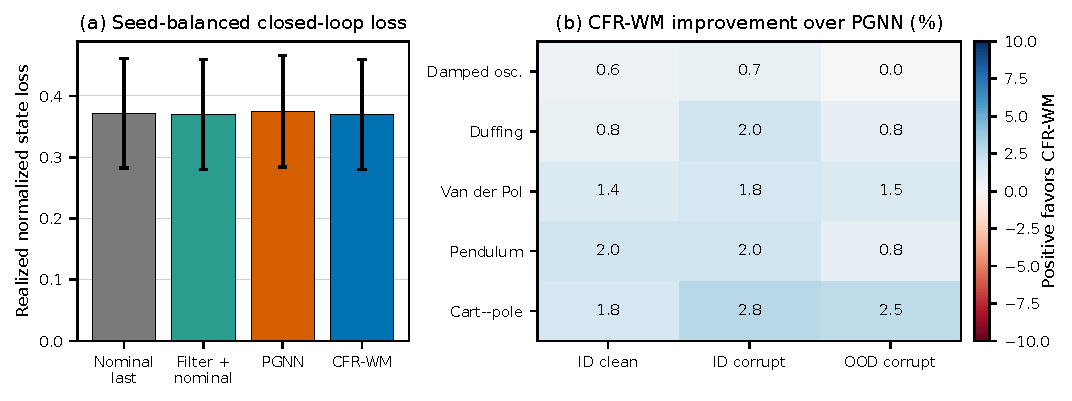
\includegraphics[width=0.92\textwidth]{figures/FigClosedLoop.pdf}
  \caption{Frozen closed-loop study. (a) Seed-balanced mean normalized state
  loss; error bars are one SD across eight seeds. (b) Mean CFR-WM improvement
  over PGNN-style within each system--condition cell. Positive values favor
  CFR-WM.}
  \label{fig:closed-loop}
\end{figure*}

The absolute separation between learned predictors is small. Filter plus
nominal dynamics obtains state loss \ClosedLoopFilterNominalLoss{}, slightly
below CFR-WM's \ClosedLoopCFRLoss{}, and also uses less action effort (0.398
versus 0.404). The nominal-last interface reaches \ClosedLoopNominalLoss{}.
Closed-loop performance therefore supports the value of context correction,
but not an additional benefit from the learned residual.

\subsection{Measured-flight transfer}

On held-out NanoDrone flights, CFR-WM improves 50-step position RMSE over the
matched unfiltered residual model in all four context conditions
(Table~\ref{tab:external-position}). For example, under combined noise and
missingness, position RMSE is $0.094\pm0.004$ m versus
$0.125\pm0.017$ m. The state components do not move uniformly: the unfiltered
model has lower 50-step full-state NRMSE in all eight context--horizon
comparisons, and it has lower velocity error for recorded and missing-only
contexts.

\begin{table*}[!t]
  \caption{External 50-step physical errors on three held-out NanoDrone
  flights. Entries are mean $\pm$ SD across five training seeds after equal
  weighting of flights.}
  \label{tab:external-position}
  \centering
  \footnotesize
  \begin{tabular}{lrrrr}
\toprule
& \multicolumn{2}{c}{Position RMSE (m)} & \multicolumn{2}{c}{Velocity RMSE (m/s)} \\
Context & CFR-WM & Unfiltered & CFR-WM & Unfiltered \\
\midrule
As recorded & $0.078 \pm 0.003$ & $0.083 \pm 0.010$ & $0.249 \pm 0.015$ & $0.233 \pm 0.009$ \\
Noise & $0.091 \pm 0.003$ & $0.115 \pm 0.007$ & $0.257 \pm 0.014$ & $0.258 \pm 0.007$ \\
Missing & $0.081 \pm 0.005$ & $0.095 \pm 0.022$ & $0.259 \pm 0.014$ & $0.243 \pm 0.009$ \\
Noise + missing & $0.094 \pm 0.004$ & $0.125 \pm 0.017$ & $0.267 \pm 0.014$ & $0.268 \pm 0.009$ \\
\bottomrule
\end{tabular}

\end{table*}

The probabilistic output is not calibrated for this transfer. CFR-WM's nominal
90\% marginal coverage ranges from 0.524 to 0.667 across the four context
conditions, compared with 0.565--0.779 for the matched unfiltered model. The
same CFR-WM intervals are narrower and have higher calibration error in every
condition. These intervals are therefore not used in the MPC objective.
